%% packages
\documentclass{article}
\usepackage[a4paper, left=2.0cm, right=2.0cm, top=3.5cm]{geometry}
\usepackage[ngerman]{babel}
\usepackage{graphicx}
\usepackage{multicol}
\usepackage{amssymb}
\usepackage{titlesec}
\usepackage{wrapfig}
\usepackage{blindtext}
\usepackage{lipsum}
\usepackage{caption}
\usepackage{listings}
\usepackage{fancyhdr}
\usepackage{nopageno}
\usepackage{authblk}
\usepackage{amsmath} % tons of math stuff
\usepackage{mathtools} % e.g. alignment within matrix
%\usepackage{bm} % provides shorthand for bold in math mode
\usepackage{dsfont} % \mathds makes double stroke digits
\usepackage{esdiff} % provides derivative commands
%\usepackage[ISO]{diffcoeff}
\usepackage{xcolor}
\usepackage{csquotes} % e.g. provides \enquote
\usepackage[separate-uncertainty=true]{siunitx} % units
\usepackage{xcolor} % colored text
%\fancyhf[]{}
\usepackage{csvsimple}


%% custom stuff
% own units
\DeclareSIUnit \VSS {\ensuremath{V_\mathrm{SS}}}
\DeclareSIUnit \VS {\ensuremath{V_\mathrm{S}}}
\DeclareSIUnit \Veff {\ensuremath{V_\mathrm{eff}}}
\DeclareSIUnit \Vpp {\ensuremath{V_\mathrm{pp}}}
\DeclareSIUnit \Vp {\ensuremath{V_\mathrm{p}}}
\DeclareSIUnit \VRMS {\ensuremath{V_\mathrm{RMS}}}
\DeclareSIUnit \ASS {\ensuremath{A_\mathrm{SS}}}
\DeclareSIUnit \AS {\ensuremath{A_\mathrm{S}}}
\DeclareSIUnit \Aeff {\ensuremath{A_\mathrm{eff}}}
\DeclareSIUnit \App {\ensuremath{A_\mathrm{pp}}}
\DeclareSIUnit \Ap {\ensuremath{A_\mathrm{p}}}
\DeclareSIUnit \ARMS {\ensuremath{A_\mathrm{RMS}}}

% change subsection numbering to capital letters
\newcommand{\subsectionAlph}{ \renewcommand{\thesubsection}{\arabic{section}.\Alph{subsection}} }
% change subsection numbering to lowercase letters
\newcommand{\subsectionalph}{ \renewcommand{\thesubsection}{\arabic{section}.\alph{subsection}} }

% own fig. that works with multicols
\newenvironment{Figure}
  {\par\medskip\noindent\minipage{\linewidth}}
  {\endminipage\par\medskip}
\newcommand*{\inputPath}{./plot} % prepend this command to the argument of all input commands
\graphicspath{ {./images/} }

% own commands
% \newcommand{\rarr}{$\to\,$} %A$\,\to\,$B
\newcommand{\defc}{black}
\newcommand{\colorT}[2][blue]{\color{#1}{#2}\color{\defc}}
\newcommand{\redq}{\color{red}(?)\color{\defc}}
\newcommand{\question}[1]{\colorT[purple]{(#1)}}
\newcommand{\todo}[1]{\colorT[red]{\textbf{(#1)}}}
\newcommand{\mr}{\mathrm}


%% preparation
\begin{titlepage}
    \title{Elektronikpraktikum: Versuch 0 \\ Einführungsversuch}
    \author[1]{Marc Hauer\thanks{s65mhaue@uni-bonn.de}}
    \author[1]{Michael Vogt\thanks{s65mvogt@uni-bonn.de}}
    \affil[1]{Uni Bonn}
    %\date{\today}
\end{titlepage}


%% document
\begin{document}

\pagenumbering{gobble}
\maketitle
\tableofcontents
\newpage
\pagenumbering{arabic}

\pagestyle{fancy}
\fancyhead[R]{\thepage}
\fancyhead[L]{\leftmark}

%\begin{multicols}{2}

\section*{Einleitung}
Versuch 0 dient zum kennenlernen der im Elektronikpraktikum eingesetzten Gerätschaften und führt in ihre Eigenheiten ein.
Im Zuge dessen betrachten wir mit dem Oszilloskop verschiedene durch einen Funktionsgenerator erzeugte Signalformen,
und untersuchen Anstiegszeit und Grenzfrequenz des Generators.

\section{Theorie}
\subsection{Charakterisierung von Wechselspannungen}
Bei Wechselspannungssignalen liegt keine schlicht konstante, sondern eine periodisch variierende Spannung vor.
Daher gibt es verschiedene Möglichkeiten, das Signal durch einen Wert zu charakterisieren.
Diese Spannungsangaben werden durch einen Index am Formelzeichen $U_X$ oder an der Einheit Volt $V_X$ gekennzeichnet.
\begin{description} 
  \item[Spitze-Spitze] $U_\mathrm{pp}$ (peak-to-peak) entspricht der Differenz zwischen
  dem höchsten und niedrigsten auftretenden Spannungswert.
  \item[Scheitelwert / Spitzenwert] $U_\mathrm{p}$ gibt den maximalen auftretenden Spannungswert an. Bei asymmetrischen Signalen
  ist damit meist, aber nicht immer, $U_\mathrm{p} = \max{\lvert U(t) \rvert}$ gemeint.
  \item[Effektivwert] $U_\mathrm{eff}$ entspricht der Gleichspannung, welche die gleiche mittlere Leistung über einen Widerstand
  $R$ verrichtet, wie das eigentliche Signal. Mit $P=U^2/R$ muss also $U_\mathrm{eff} = \sqrt{\langle U^2 \rangle_t}$.
  $U_\mathrm{eff}$ ist also die \textit{root mean square}-Spannung und wird auch als $U_\mathrm{RMS}$ geschrieben.
\end{description} 

\subsection{Funktionsgenerator}
Um Wechselspannungen verschiedener Formen zu produzieren, verwenden wir den Funktionsgenerator HM 8131-2,
welcher einen Ausgangswiderstand von $50\Omega$ hat. Es ist zu beachten, dass das Gerät eine endliche
Frequenzbandbreite hat, welche sich hier durch einen RC-Tiefpass beschreiben lässt, dessen Grenzfrequenz der
Bandbreite entspricht:
\begin{equation}
  B = f_\text{grenz} = 1/(2\pi RC) = 1 / (2\pi \tau) \quad \text{mit Zeitkonstante } \tau = RC
\end{equation}
Bei zeitlicher Darstellung des Signals zeigt sich diese Frequenzbegrenzung in Form einer endlichen Anstiegszeit $\Delta t$ bei abrupten
Spannungsänderungen (beispielsweise würde ein perfektes Rechtecksignal unendlich hohe Frequenzen benötigen). $\Delta t$ wird definiert
als Zeitdifferenz zwischen dem Erreichen von $10 \%$ und $ 90\%$ der Maximalspannung. Es gilt näherungsweise
\begin{equation}
  B \Delta t = 0.35 \label{eq:bdeltat}
\end{equation}

\subsection{Oszilloskop}
Das Oszilloskop ist ein wichtiges Instrument zur Messung periodischer Signale. Bei einem analogen Oszilloskop
(wie dem früher im Praktikum verwendeten HAMEG HM604)
besteht die Anzeige aus einer Elektronenstrahlröhre mit Leuchtschirm. Der Elektronenstrahl kann durch zwei Plattenkondensatoren,
deren Felder in $x$- (horizontal) bzw. $y$-Richtung (vertikal) zeigen, gesteuert werden. Meist wird an die x-Platten
eine zeitlich gleichförmig steigende Spannung, und an die y-Platten das darzustellende Signal angelegt. So entsteht als
Oszillogramm ein \enquote{Plot} des Signals gegen die Zeit.

Die steigende x-Spannung wird durch Integration einer konstanten Spannung
und Rücksetzung auf einen Ausgangswert durch ein Triggersignal erreicht. Dieser Trigger kann von dem y-Signal abhängig
gemacht werden, um die Periodizität von x- und y- Signal aneinander anzupasssen. Nur so entsteht ein
(scheinbar, bei Betrachtung mit bloßem Auge) zeitlich unveränderliches Oszillogramm.

Das Oszilloskop hat eine Eingansimpedanz, die durch einen Widerstand von $1\mathrm{\Omega}$ in Parallelschaltung zu
einer Kapazität von ca. $30\mathrm{pF}$ entsteht. Die Eingangsimpedanz kann häufig als unendlich genähert werden.

Wie auch der Funktionsgenerator, hat das Oszilloskop ebenfalls eine endliche Bandbreite B. Bei Messung der Anstiegszeit
wird somit ein höherer Wert gemessen, nach der Formel
\begin{equation}
  \Delta t^2_\text{gemessen} = \Delta t^2_\text{Signal} + \Delta t^2_\text{Oszi} \label{eq:anstiegszeit-eff}
\end{equation}


\section{Voraufgaben}
\begingroup
%\refstepcounter{subsection}
\subsectionAlph
\subsection{}
Für eine Sinusförmige Spannung der Frequenz $\omega$ und Amplitude $U_0$ gilt $U_\text{SS} = 2U_0$ und $U_\text{S} = U_0$.
Und für den Effektivwert
\begin{equation}
  U_\text{eff} = \sqrt{\langle U^2 \rangle} = U_0 \sqrt{\frac{w}{2\pi} \int_0^{2\pi/\omega} dt \sin^2(\omega t)} = U_0/\sqrt{2}
\end{equation}

\subsection{}
Für ein symmetrisches Rechtecksignal mit $U_\text{S} = 10\text{V}$ gilt $U^2 = U_\text{S}^2 = \text{const.}$
Damit ist $U_\text{eff} = \sqrt{\langle U^2 \rangle} = \lvert U_\text{S} \rvert = 10\text{V}$

\subsection{}
Es gilt $U_n = U_0 \frac{R_n}{R_n+R_i}$ mit $n=1,\enspace 2$ und damit
\begin{align}
  \frac{U_2 - U_1}{I_1 - I_2} &= \frac{ \frac{R_2}{R_2+R_i} - \frac{R_1}{R_1+R_i}}{ \frac{1}{R_1+R_i} - \frac{1}{R_2+R_i} } \nonumber \\ 
  &= \frac{ R_2(R_1+R_i) - R_1(R_2+R_i) }{ (R_2+R_i) - (R_1+R_i) } = \frac{R_i(R_2-R_1)}{R_2-R_1} = R_i
\end{align}
Der Signalgenerator liefert $20\text{V}_\text{SS}$ ohne Last, also mit $I_1$=0, und $\SI{10}{\VSS}$ mit $50\mathrm{\Omega}$ Last,
also $I_2 = \frac{U_2}{R_2} = 0.2A_\text{SS}$. damit gilt $R_i = \frac{U_2 - U_1}{I_1 - I_2} = 50\mathrm{\Omega}$.

\subsection{}
Wir machen uns mit den Bedienungselementen des Oszilloskops vertraut.

\subsection{}
Wir leiten (\ref{eq:bdeltat}) her. Für die exponentiell auf Spannung $U_0$ ansteigende Flanke gilt
%\begin{align*}
%  U(t) &= U_0 - \exp(-\frac{t}{\tau}) \\
%  \implies t(U) &= -\tau \ln(U_0 - U) \\
%  \implies \Delta t &= t(0.9 U_0) - t(0.1 U_0) = \tau \ln(\frac{U_0-0.1U_0}{U_0-0.9U_0}) = \tau \ln(9) \\
%  \implies B \Delta t &= \frac{1}{2\pi\tau} \cdot \tau \cdot \ln(9) \approx 0.35
%\end{align*}
\begin{align*}
  U(t) &= U_0 \left(1 - \exp(-\frac{t}{\tau})\right) \\
  \implies t(U) &= -\tau \ln\left(1 - \frac{U}{U_0}\right) = -\tau \ln\left(\frac{U_0-U}{U_0}\right) \\
  \implies \Delta t &= t(0.9 U_0) - t(0.1 U_0) = \tau \ln\left(\frac{U_0-0.1U_0}{U_0-0.9U_0}\right) = \tau \ln(9) \\
  \implies B \Delta t &= \frac{1}{2\pi\tau} \cdot \tau \cdot \ln(9) \approx 0.35
\end{align*}

\endgroup

\section{Durchführung \& Auswertung}
\begingroup
\subsectionalph

\subsection{}
Um den Signalgenerator und das Oszilloskop kennenzulernen, verbinden wir diese mit einem Koaxialkabel (BNC-Kabel)
und erzeugen mit dem Generator verschiedene Signale, die wir dann mit dem Oszi beobachten.

\subsection{}
Zur Messung der insgesamten Anstiegszeit erzeugen wir ein Rechtecksignal mit einer Frequenz von $\SI{2}{\mega\hertz}$ und $\SI{20}{\Vpp}$. Wir nutzen das Oszi um die $10\%$ und $90\%$ des Signalmaximums zu ermitteln und speichern das Bild mit diesen Hilfslinien (Abb. \ref{fig:anstiegszeit}).

\begin{figure}
    \centering
    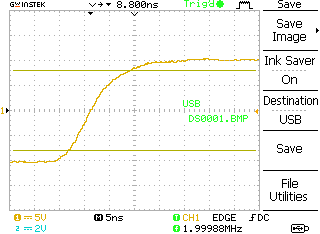
\includegraphics[width=0.6\linewidth]{b2}
    \caption{Oszillogramm des \SI{2}{\MHz}-Rechtecksignals.}
    \label{fig:anstiegszeit}
\end{figure}

Daraus lässt sich die Anstiegszeit $\Delta t_\text{gemessen}$ ablesen.
Die $10\%$-Linie wird bei $t_{10}=\SI{-13\pm1}{\ns}$ und die $90\%$-Linie bei $t_{90}=\SI{-1\pm1}{\ns}$ erreicht. Damit ergibt sich
\begin{equation}
    \Delta t_\mr{gemessen} = t_{90}-t_{10} = \SI{12\pm1.41}{\ns}
\end{equation}
Die tatsächliche Anstiegszeit des Signals $\Delta t_\text{Signal}$ erhalten wir dann über $\Delta t_\text{Oszi}$, was sich aus der Bandbreite des Oszilloskops $B_\text{Oszi} = \SI{70}{\mega\hertz}$ ergibt
\begin{equation}
    \Delta t_\text{Ozsi} = \frac{0.35}{B_\text{Oszi}} = \frac{0.35}{\SI{70}{\mega\hertz}} = \SI{5}{\ns}
\end{equation}
aus (\ref{eq:anstiegszeit-eff}) folgt
\begin{align}
    \Delta t_\mr{Signal} &= \sqrt{\Delta t_\mr{gemessen}^2 - \Delta t_\mr{Oszi}^2} \\
    \Delta(\Delta t_\mr{Signal}) &= \frac{1}{2} (\Delta t_\mr{gemessen}^2 - \Delta t_\mr{Oszi}^2)^{-\frac{1}{2}} \cdot 2 \Delta t_\mr{gemessen} \Delta(\Delta t_\mr{gemessen}) \nonumber \\
    &= \frac{\Delta t_\mr{gemessen}}{\Delta t_\mr{Signal}} \cdot \Delta(\Delta t_\mr{gemessen})
\end{align}
und wir erhalten $\Delta t_\mr{Signal} = \SI{10.91\pm1.56}{\ns}$.

Damit lässt sich auch die Bandbreite des Signalgenerators $B_\text{Signal}$ ermitteln:
\begin{align}
    B_\text{Signal} &= \frac{0.35}{\Delta t_\text{Signal}} \\
    \Delta B_\text{Signal} &= \frac{0.35}{(\Delta t_\text{Signal})^2}\cdot \Delta(\Delta t_\text{Signal})
\end{align}
Es ergibt sich $B_\mr{Signal} = \SI{32.08 \pm 4.59}{\MHz}$.


\subsection{}
Anschließend schalten wir einen RC-Filter ($R=\SI{390}{\ohm}$, $C=\SI{0.1}{\micro\farad}$) zwischen den Ausgang des Signalgenerators und den Eingang des Oszilloskops.
Für verschiedene Frequenzen eines $U_0 = \SI{20}{\Vpp}$-Sinussignals messen wir die über dem
Kondensator abgegriffene resultierende Amplitude $U$, um die Dämpfung durch den Filter zu bestimmen (Abb. \ref{fig:bode}).

Die Grenzfrequenz ist die Frequenz, bei der $\frac{U}{U_0}=\frac{1}{\sqrt{2}}$ ist, also die Dämpfung $20\log(\frac{1}{\sqrt{2}}) \approx -3 \unit{\dB}$ ist. Der Schnittpunkt mit dieser Linie liegt bei $f_\mr{Grenz} = \SI{3650 \pm 50}{\Hz}$

\begin{figure}
    \centering
    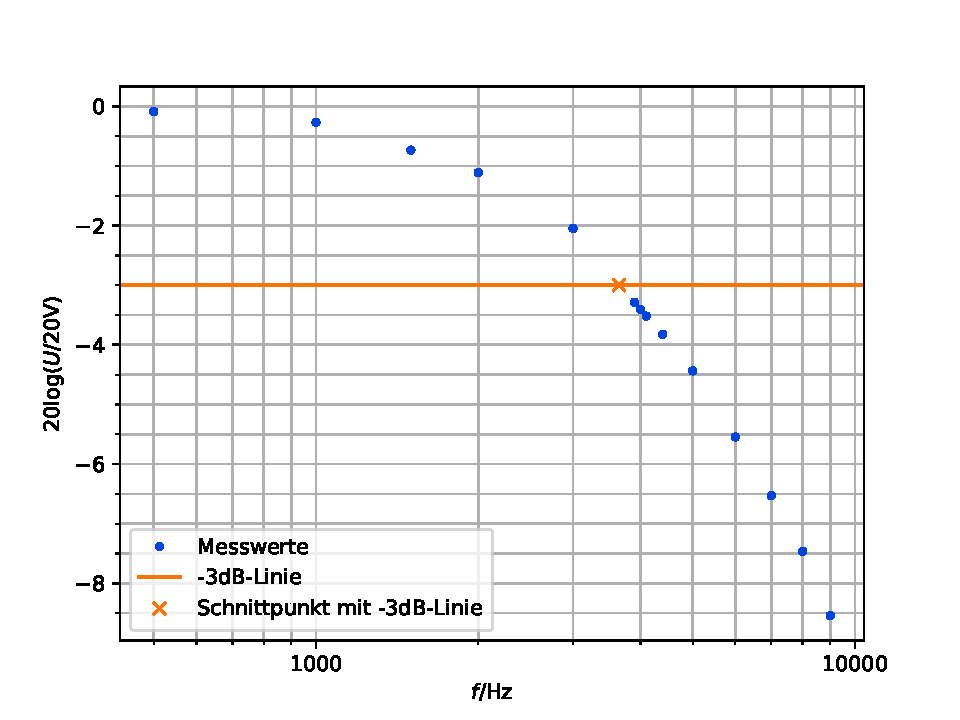
\includegraphics[width=0.75\linewidth]{c}
    \caption{Bode Diagramm des RC-Tiefpassfilters. $f$ ist die Frequenz des Signals und $U$ die Amplitude der Ausgangsspannung. Werte siehe Tab.\ref{tab:bode}.}
    \label{fig:bode}
\end{figure}

\begin{table}[]
    \centering
    \csvreader[
        head to column names,
        tabular=|c|c|,
        table head=\hline \textbf{f/Hz} & \textbf{U\_pp/V} \\ \hline,
        late after line=\\\hline
    ]{data/c.csv}{}
    {\csname f/Hz\endcsname & \csname U_pp/V\endcsname}
    \caption{}
    \label{tab:bode}
\end{table}


%(in \unit{\decibel}) gegen die Frequenz aufzutragen.

\endgroup

%\end{multicols}
\end{document}
